\documentclass{standalone}
\usepackage{tikz}
\usetikzlibrary{patterns, positioning}


\begin{document}
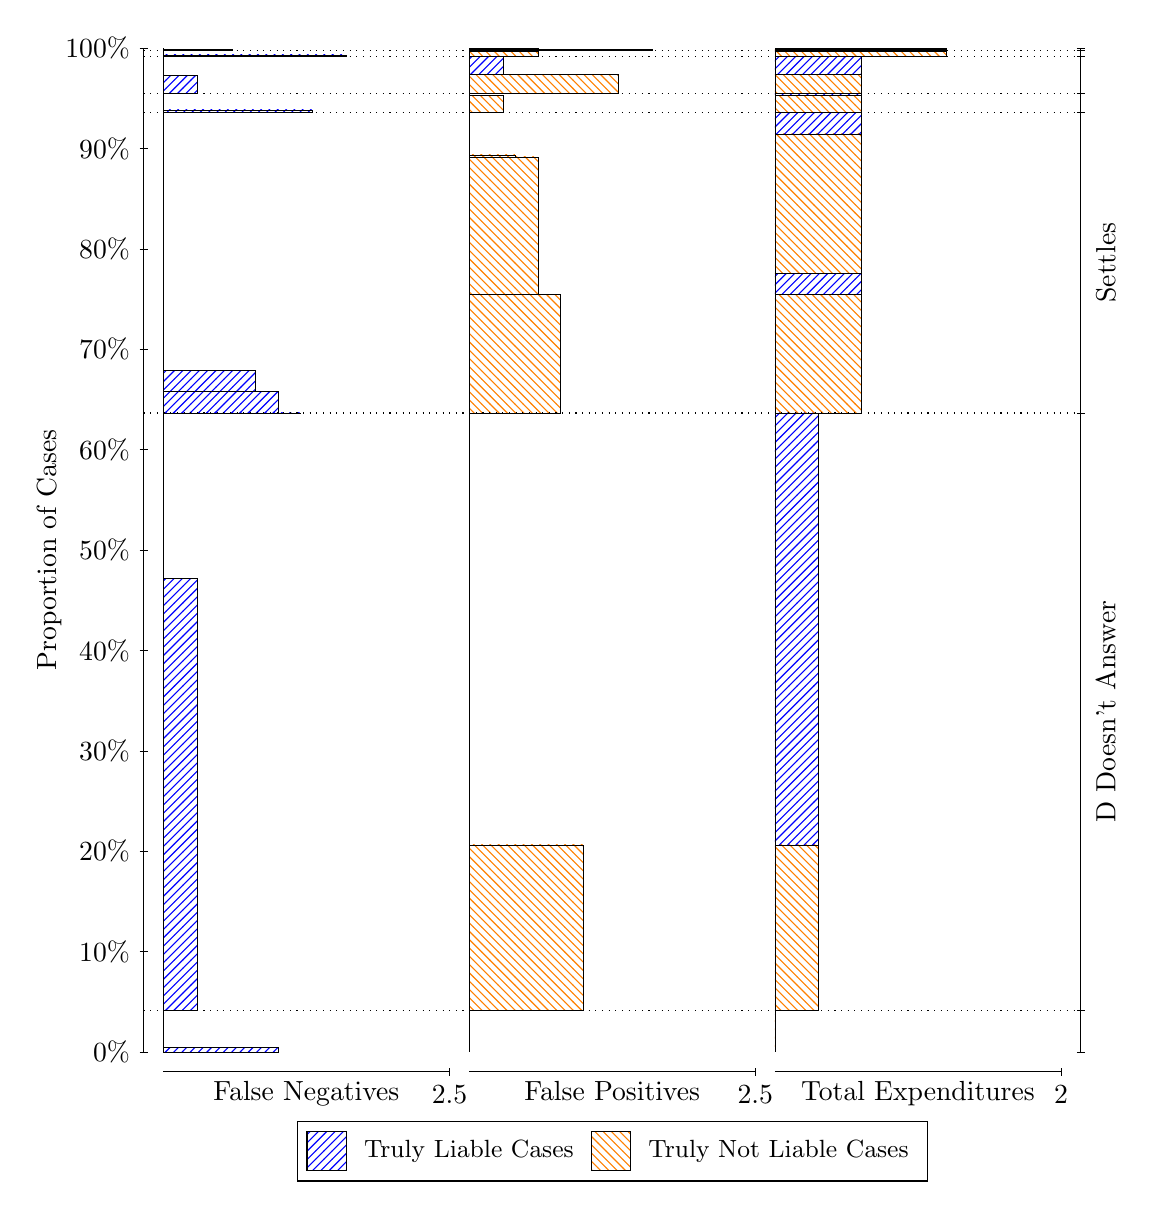
\begin{tikzpicture}
\draw[black, very thin] (1.5,1.75) -- (1.5,14.5);
\node[rotate=90, text=black, anchor=center] at (0.3, 8.125) {Proportion of Cases};
\draw[black, very thin] (1.45,1.75) -- (1.55,1.75);
\node[text=black, anchor=east] at (1.45, 1.75) {0\%};
\draw[black, very thin] (1.45,3.025) -- (1.55,3.025);
\node[text=black, anchor=east] at (1.45, 3.025) {10\%};
\draw[black, very thin] (1.45,4.3) -- (1.55,4.3);
\node[text=black, anchor=east] at (1.45, 4.3) {20\%};
\draw[black, very thin] (1.45,5.575) -- (1.55,5.575);
\node[text=black, anchor=east] at (1.45, 5.575) {30\%};
\draw[black, very thin] (1.45,6.85) -- (1.55,6.85);
\node[text=black, anchor=east] at (1.45, 6.85) {40\%};
\draw[black, very thin] (1.45,8.125) -- (1.55,8.125);
\node[text=black, anchor=east] at (1.45, 8.125) {50\%};
\draw[black, very thin] (1.45,9.4) -- (1.55,9.4);
\node[text=black, anchor=east] at (1.45, 9.4) {60\%};
\draw[black, very thin] (1.45,10.675) -- (1.55,10.675);
\node[text=black, anchor=east] at (1.45, 10.675) {70\%};
\draw[black, very thin] (1.45,11.95) -- (1.55,11.95);
\node[text=black, anchor=east] at (1.45, 11.95) {80\%};
\draw[black, very thin] (1.45,13.225) -- (1.55,13.225);
\node[text=black, anchor=east] at (1.45, 13.225) {90\%};
\draw[black, very thin] (1.45,14.5) -- (1.55,14.5);
\node[text=black, anchor=east] at (1.45, 14.5) {100\%};

\draw[black, very thin] (13.4,1.75) -- (13.4,14.5);
\draw[black, very thin] (13.35,1.75) -- (13.45,1.75);
\node[anchor=west] at (13.35, 1.75) {};
\draw[black, very thin] (13.35,2.2772) -- (13.45,2.2772);
\node[anchor=west] at (13.35, 2.2772) {};
\draw[black, very thin] (13.35,9.8651) -- (13.45,9.8651);
\node[anchor=west] at (13.35, 9.8651) {};
\draw[black, very thin] (13.35,13.684) -- (13.45,13.684);
\node[anchor=west] at (13.35, 13.684) {};
\draw[black, very thin] (13.35,13.925) -- (13.45,13.925);
\node[anchor=west] at (13.35, 13.925) {};
\draw[black, very thin] (13.35,14.397) -- (13.45,14.397);
\node[anchor=west] at (13.35, 14.397) {};
\draw[black, very thin] (13.35,14.469) -- (13.45,14.469);
\node[anchor=west] at (13.35, 14.469) {};
\draw[black, very thin] (13.35,14.5) -- (13.45,14.5);
\node[anchor=west] at (13.35, 14.5) {};

\draw[black, very thin, pattern color=blue, pattern=north east lines] (1.75,1.75) rectangle (3.2033,1.8055);
\draw[black, very thin, pattern color=orange, pattern=north west lines] (1.75,1.8055) rectangle (1.75,2.2772);
\draw[black, very thin, pattern color=blue, pattern=north east lines] (1.75,2.2772) rectangle (2.186,7.762);
\draw[black, very thin, pattern color=orange, pattern=north west lines] (1.75,7.762) rectangle (1.75,9.8651);
\draw[black, very thin, pattern color=blue, pattern=north east lines] (1.75,9.8651) rectangle (3.494,9.8677);
\draw[black, very thin, pattern color=blue, pattern=north east lines] (1.75,9.8677) rectangle (3.2033,10.14);
\draw[black, very thin, pattern color=blue, pattern=north east lines] (1.75,10.14) rectangle (2.9127,10.407);
\draw[black, very thin, pattern color=orange, pattern=north west lines] (1.75,10.407) rectangle (1.75,13.684);
\draw[black, very thin, pattern color=blue, pattern=north east lines] (1.75,13.684) rectangle (3.6393,13.714);
\draw[black, very thin, pattern color=orange, pattern=north west lines] (1.75,13.714) rectangle (1.75,13.925);
\draw[black, very thin, pattern color=blue, pattern=north east lines] (1.75,13.925) rectangle (2.186,14.157);
\draw[black, very thin, pattern color=orange, pattern=north west lines] (1.75,14.157) rectangle (1.75,14.397);
\draw[black, very thin, pattern color=blue, pattern=north east lines] (1.75,14.397) rectangle (4.0753,14.413);
\draw[black, very thin, pattern color=orange, pattern=north west lines] (1.75,14.413) rectangle (1.75,14.469);
\draw[black, very thin, pattern color=blue, pattern=north east lines] (1.75,14.469) rectangle (2.622,14.484);
\draw[black, very thin, pattern color=orange, pattern=north west lines] (1.75,14.484) rectangle (1.75,14.5);
\draw[black, very thin, pattern color=orange, pattern=north west lines] (5.6333,1.75) rectangle (5.6333,2.2217);
\draw[black, very thin, pattern color=blue, pattern=north east lines] (5.6333,2.2217) rectangle (5.6333,2.2772);
\draw[black, very thin, pattern color=orange, pattern=north west lines] (5.6333,2.2772) rectangle (7.0867,4.3803);
\draw[black, very thin, pattern color=blue, pattern=north east lines] (5.6333,4.3803) rectangle (5.6333,9.8651);
\draw[black, very thin, pattern color=orange, pattern=north west lines] (5.6333,9.8651) rectangle (6.796,11.374);
\draw[black, very thin, pattern color=orange, pattern=north west lines] (5.6333,11.374) rectangle (6.5053,13.117);
\draw[black, very thin, pattern color=orange, pattern=north west lines] (5.6333,13.117) rectangle (6.2147,13.142);
\draw[black, very thin, pattern color=blue, pattern=north east lines] (5.6333,13.142) rectangle (5.6333,13.684);
\draw[black, very thin, pattern color=orange, pattern=north west lines] (5.6333,13.684) rectangle (6.0693,13.895);
\draw[black, very thin, pattern color=blue, pattern=north east lines] (5.6333,13.895) rectangle (5.6333,13.925);
\draw[black, very thin, pattern color=orange, pattern=north west lines] (5.6333,13.925) rectangle (7.5227,14.165);
\draw[black, very thin, pattern color=blue, pattern=north east lines] (5.6333,14.165) rectangle (6.0693,14.397);
\draw[black, very thin, pattern color=orange, pattern=north west lines] (5.6333,14.397) rectangle (6.5053,14.453);
\draw[black, very thin, pattern color=blue, pattern=north east lines] (5.6333,14.453) rectangle (5.6333,14.469);
\draw[black, very thin, pattern color=orange, pattern=north west lines] (5.6333,14.469) rectangle (7.9587,14.485);
\draw[black, very thin, pattern color=blue, pattern=north east lines] (5.6333,14.485) rectangle (6.5053,14.5);
\draw[black, very thin, pattern color=orange, pattern=north west lines] (9.5167,1.75) rectangle (9.5167,2.2217);
\draw[black, very thin, pattern color=blue, pattern=north east lines] (9.5167,2.2217) rectangle (9.5167,2.2772);
\draw[black, very thin, pattern color=orange, pattern=north west lines] (9.5167,2.2772) rectangle (10.062,4.3803);
\draw[black, very thin, pattern color=blue, pattern=north east lines] (9.5167,4.3803) rectangle (10.062,9.8651);
\draw[black, very thin, pattern color=orange, pattern=north west lines] (9.5167,9.8651) rectangle (10.607,11.374);
\draw[black, very thin, pattern color=blue, pattern=north east lines] (9.5167,11.374) rectangle (10.607,11.641);
\draw[black, very thin, pattern color=orange, pattern=north west lines] (9.5167,11.641) rectangle (10.607,13.409);
\draw[black, very thin, pattern color=blue, pattern=north east lines] (9.5167,13.409) rectangle (10.607,13.684);
\draw[black, very thin, pattern color=orange, pattern=north west lines] (9.5167,13.684) rectangle (10.607,13.895);
\draw[black, very thin, pattern color=blue, pattern=north east lines] (9.5167,13.895) rectangle (10.607,13.925);
\draw[black, very thin, pattern color=orange, pattern=north west lines] (9.5167,13.925) rectangle (10.607,14.165);
\draw[black, very thin, pattern color=blue, pattern=north east lines] (9.5167,14.165) rectangle (10.607,14.397);
\draw[black, very thin, pattern color=orange, pattern=north west lines] (9.5167,14.397) rectangle (11.697,14.453);
\draw[black, very thin, pattern color=blue, pattern=north east lines] (9.5167,14.453) rectangle (11.697,14.469);
\draw[black, very thin, pattern color=orange, pattern=north west lines] (9.5167,14.469) rectangle (11.697,14.485);
\draw[black, very thin, pattern color=blue, pattern=north east lines] (9.5167,14.485) rectangle (11.697,14.5);
\draw[black, dotted] (1.5,2.2772) -- (13.4,2.2772);
\draw[black, dotted] (1.5,9.8651) -- (13.4,9.8651);
\draw[black, dotted] (1.5,13.684) -- (13.4,13.684);
\draw[black, dotted] (1.5,13.925) -- (13.4,13.925);
\draw[black, dotted] (1.5,14.397) -- (13.4,14.397);
\draw[black, dotted] (1.5,14.469) -- (13.4,14.469);
\draw[black, very thin] (1.75,1.5) -- (5.3833,1.5);
\node[text=black, anchor=north] at (3.5667, 1.5) {False Negatives};
\draw[black, very thin] (5.3833,1.45) -- (5.3833,1.55);
\node[text=black, anchor=north] at (5.3833, 1.45) {2.5};

\draw[black, very thin] (5.6333,1.5) -- (9.2667,1.5);
\node[text=black, anchor=north] at (7.45, 1.5) {False Positives};
\draw[black, very thin] (9.2667,1.45) -- (9.2667,1.55);
\node[text=black, anchor=north] at (9.2667, 1.45) {2.5};

\draw[black, very thin] (9.5167,1.5) -- (13.15,1.5);
\node[text=black, anchor=north] at (11.333, 1.5) {Total Expenditures};
\draw[black, very thin] (13.15,1.45) -- (13.15,1.55);
\node[text=black, anchor=north] at (13.15, 1.45) {2};


\node[text=black, centered, rotate=90] at (13.72, 6.0711) {D Doesn't Answer};
\node[text=black, centered, rotate=90] at (13.72, 11.775) {Settles};





\draw (7.449999999999999,1.5) node[draw=none] (baseCoordinate) {};
\begin{scope}[align=center]
        \matrix[scale=0.5, draw=black, below=0.5cm of baseCoordinate, nodes={draw}, column sep=0.1cm]{
            \node[rectangle, draw, minimum width=0.5cm, minimum height=0.5cm, pattern color=blue, pattern=north east lines] {}; &
            \node[draw=none, font=\small, text=black] (B) {Truly Liable Cases}; &
            \node[rectangle, draw, minimum width=0.5cm, minimum height=0.5cm, pattern color=orange, pattern=north west lines] {}; &
            \node[draw=none, font=\small, text=black] (B) {Truly Not Liable Cases}; \\
            };
\end{scope}

\end{tikzpicture}
\end{document}